\chapter{Implementation des Simplex Algorithmus}
\rhead{Implementation des Simplex Algorithmus}
\chapterauthor{Andreas M"uller}

Der Simplex Algorithmus basiert auf Operationen, die man typischerweise
vom Gaussschen Eliminationsalgorithmus her kennt.
Trotzdem bieten die "ublichen Bibliotheken f"ur lineare Algebra,
wie zum Beispiel LAPACK, keine direkt auf lineare Optimierung
ausgelegten Funktionen.
In diesem Abschnitt wird daher dargestellt, wie man den Simplex-Algorithmus
implementieren und trotzdem von der Performance solcher
Bibliotheken profitieren kann.

\section{Eine genauere Analyse der Operationen}
Das Standard-Optimierungs-Problem mit nicht negativen Variablen $x_i\ge 0$
dem Nullpunkt als zul"assigem Punkt braucht zur L"osung nur zwei Schritte,
die iteriert werden m"ussen:
\begin{enumerate}
\item Auswahl des Pivot-Elementes.
\item Austauschoperation.
\end{enumerate}
Die Auswahl des Pivot-Elementes verwendet eine Strategie, f"ur welche es
bei der L"osung linearer Gleichungssystemen nichts vergleichbares gibt.
Sowohl bei der Wahl der Spalten wie auch der Zeilen muss man Elemente 
w"ahlen, welche welche eine Extremalbedingung erf"ullen. Ausserdem
darf nur eine Pivot-Spalte gew"ahlt werden, welche aktuell als
frei w"ahlbar markiert ist. Diese Operation muss also vollst"andig neu
implementiert werden.

Die Austausch-Operation ist eigentlich eine Zeilen-Operation mit der
Pivot-Zeile durch die alle Elemente der Pivot-Spalte bis auf die Eins
in der Pivot-Zeile eliminiert werden. Diese Operation wird auch
bei der L"osung lienarer Gleichungssysteme immer wieder durchgef"uhrt,
sowohl beim Vorw"artsreduzieren als auch beim R"uckw"artseinsetzen.
Allerdings werden dort viele solche Operationen kombiniert, f"ur sich
allein genommen ist die Operation nicht sehr interessant.

Die Austausch-Operation besteht genauer aus folgenden Schritten:
\begin{enumerate}
\item Division der Pivot-Zeile durch das Pivot-Element.
\item Subtraktion eines Vielfachen der (neuen) Pivot-Zeile von allen
Zeilen ausser der Pivot-Zeile.
\end{enumerate}
Die Reihenfolge ist kritisch, es muss sichergestellt sein, dass die
Pivot-Division abgeschlossen ist, bevor ein Element der Pivot-Zeile
f"ur Schritt 2 verwendet wird.

\section{Implementationsm"oglichkeiten f"ur die Austausch-Operation}
Im Verzeichnis {\tt code/simplex} findet man eine Implementation
des Simplex-Algorithmus mit drei verschiedenen Techniken.
Im File {\tt backend.c} wird gezeigt, wie man die Wahl des berechnenden
Backends weitgehend transparent machen kann, so dass es einfacher wird,
vergleichende Performance-Messungen durchzuf"uhren.

\subsection{Implementation in C}
Die Implementation der Pivot-Operation ist problemlos, im Beispiel-Code
wird sie im File {\tt simplexcpu.c} implementiert.

\subsection{Implementation in OpenCL}
OpenCL ist eine aus C abgeleitete Sprache zur Formulierung paralleler
Berechnungen. Sie ist so gestaltet, dass OpenCL Code sowohl auf 
modernen Multicore CPUs als auch auf Graphikkarten ausgef"uhrt
werden kann. Letztere bieten bei leicht geringerer
Rechenleistung f"ur den Einzelthread weit h"ohere Parallelit"at an,
so dass insgesamt wesentlich gr"ossere Rechenleistung resultieren kann.

Die Verarbeitungseinheit in OpenCL ist der sogenannte Kernel.
Die Input-Daten f"ur den Kernel werden also OpenCL-Memory-Objekte
erzeugt und dann dem OpenCL-Runtime als Kernel-Parameter "ubergeben.
Der Kernel erh"alt zur Ausf"uhrungszeit ausser Pointern auf die 
Parameter auch ganzzahlige ``Koordinaten'', die "uber die
Funktionen \verb+get_global_id()+ abgerufen werden k"onnen.
Es ist also naheliegend, einen Aufruf des Kernels f"ur jedes
Matrixelement des Simplex-Tableaux zu verlangen. In jedem
Aufruf muss dann die Operation $a_{ij}-x_jy_i$
durchgef"uhrt werden, wobei $i$ und $j$ die beiden
globalen ids sind, also
\verb+get_global_id(0)+ und
\verb+get_global_id(1)+.

Mit Vorteil wird die Operation $a=a+bc$ mit der prmitiven Multiply-Accumulate
Operation {\tt fma} von OpenCL implementiert, die schneller ist und
keine Rundungsfehler der Multiplikation einf"uhrt.

Dies Aufteilung der Arbeit ist jedoch nicht unbedingt sinnvoll,
weil die pro Aufruf geleistet Arbeit sehr gering ist, es wird ja nur
gerade eine einzige {\tt fma}-Operation ausgef"uhrt.
Eine bessere L"osung, jeweils die ganze Zeilenoperation durchzuf"uhren.
Damit f"ahlt der Overhead des Aufrufs nicht mehr so stark ins Gewicht.

Ein OpenCL Device hat eine m"assig grosse Zahl von Compute Units (entspricht
etwa den Cores einer CPU), typischerweise etwa 32 Pro Graphikkarte. Jede
Compute Unit hat eine gr"ossere Zahl von Processing Elements. Eine Compute
Unit kontrolliert mehrere Processing Elements, wenn man also die
Operationen so formulieren kann, dass die gleiche Operation mit vielen
gleichartigen Datenelementen durchgef"uhrt werden muss, kann der
OpenCL Compiler eine gr"ossere Zahl von Processing Elements zum Einsatz
bringen. Man erreicht dies, indem man Vektordatentypen verwendet, 
im vorliegenden Fall {\tt double16}. Allerdings entsteht durch das 
Laden der Array-Daten also Vektor ebenfalls Overhead, so dass nicht
garantiert ist, dass sich die Laufzeit durch diesen Trick reduzieren
l"asst.

Da die Pivot-Division und die Elimination nacheinander durchgef"uhrt
werden m"ussen, muss die Arbeit in zwei Kernel aufgeteilt werden.
Denn OpenCL garantiert nur, dass die Arbeit eines Kernels vollst"andig
abgeschlossen ist, bevor der n"achste Kernel gestartet wird.
Die Beispielimplementation enth"alt dahier im File \verb+eliminate.cl+
zwei Kernel, {\tt dividerow} und {\tt eliminate}.

\subsection{BLAS}
Schreibt man die Pivot Zeile also Spaltenvektor $y$ und
die Pivotspalte als $x$, dann ist die Redukationsoperation
f"ur das Simplextableau $A$ die Operation
$ A-xy^t $, wenigstens f"ur alle Zeilen ausser der Pivot-Zeile.
Ersetzt man in $x$ und $y$ das Pivot-Element durch $0$, kann man diese 
Operation verwenden, muss aber die Pivot-Spalte anschliessen die
vom Pivot-Element verschiedenen Elemente der Pivot-Spalte separat
auf $0$ setzen.

Die Operation $A-xy^t$ ist eine Operation aus den BLAS, den
Basic Linear Algebra Subprograms.
Eine gute BLAS-Bibliothek stellt f"ur h"aufig verwendete Operationen
der numerischen linearen Algebra hochgradig optimierten Code 
zur Verf"ugung.
Auf Multicore-Maschinen und Vektor-Prozessoren werden die speziellen
F"ahigkeiten dieser Maschinen ausgenutzt, so dass man mit einer
deutlich
besseren Performance rechnen kann als mit einer Hand-Implementation.
BLAS wird soweit m"oglich von den h"oheren Funktionen von LAPACK verwendet,
so dass sie Optimierungen in BLAS auch LAPACK zu gute kommen. 

Die hier interessierende Funktion is
\begin{verbatim}
dger_(int *m, int *n, int *alpha, double *x, int *incx,
      double *y, int *incy, double *a, int *lda);
\end{verbatim}
(C-Prototyp), welche die Operation $A-\alpha $. Die Parameter haben die folgende Bedeutung:
\begin{itemize}
\item {\tt m} und {\tt n}: Dimensionen der Matrix A
\item {\tt alpha}: 
\item {\tt x}: Pivot-Zeile
\item {\tt incx}: Schritt von Element zu Element in der Spalte 
\item {\tt y}: Pivot-Spalte
\item {\tt incy}: Schritt von Element zu Element in der Zeile
\item {\tt a}: Matrix
\item {\tt lda}: f"uhrende Dimension der Matrix
\end{itemize}
Dabei ist zu beachten, dass die BLAS-Funktionen urspr"unglich in Fortran
implementiert wurden.
Fortran f"ullt einen Array spaltenweise, w"ahrend
C einen Array zeilenweise f"ullt.
Die ersten Element in einem C-Array sind also die ersten Element der
ersten Zeile, w"ahrend sie in einem Fortran-Array die erste Spalte
f"ullen. Daher wird f"ur die Anwendung im vorliegenden Fall die Rolle
von Zeile und Spalte vertauscht.

Die Implementation der Pivot-Operation ist im Beispiel-Code im
File {\tt simplexblas.c} ausgef"uhrt.

\section{Performance-"Uberlegungen}
Die Hauptarbeit bei der Durchf"uhrung des Simplex-Algorithmus wird im
Austausch-Schritt getan. Darin werden mehr als $n\times m$ Multiplikationen
und Additionen durchgef"uhrt, der Aufwand ist also $O(nm)$.
Der Aufwand f"ur die Pivot-Auswahl ist dagegen nur von der Ordnung
$O(n+m)$.

Im die Performance genauer messen zu k"onnen wurde wie folgt zuf"allig
ein Optimierungsproblem generiert. Zun"achste wurden $n$ im 
ersten Oktanten gleichverteilte Einheitsvektoren $v_i$ erzeugt.
Als Ungleichungen wurden dann die Ungleichungen $v_i^t x\le 1$ 
verwendet. Als Zielfunktion diente $x+y+z$. So erh"alt man
ein Optimierungsproblem mit $n$ Ungleichungen und $3$ Variablen.
Wegen der Gleichverteilung sind alle Simplex-Schritte ungef"ahr gleich
gross, es ist nicht mit starken Variationen von Laufzeit und
Anzahl Schritten bis zum Optimum zu rechnen. Damit eignet sich
dieses Modellproblem, um die Abh"angigkeit der Laufzeit oder
der Schrittzahl von $n$ abzusch"atzen.

\section{Resultate}
Die numerischen Experimente haben gezeigt, dass OpenCL in dieser Anwendung
keinen Vorteil bietet. Im Gegenteil: die Rechnung mit OpenCL ist
etwa dreimal langsamer als die CPU-L"osung

Am schnellsten ist die auf BLAS basierende L"osung, sie ist etwa dreimal
schneller als die naive C-Implementation.

\begin{figure}
\begin{center}
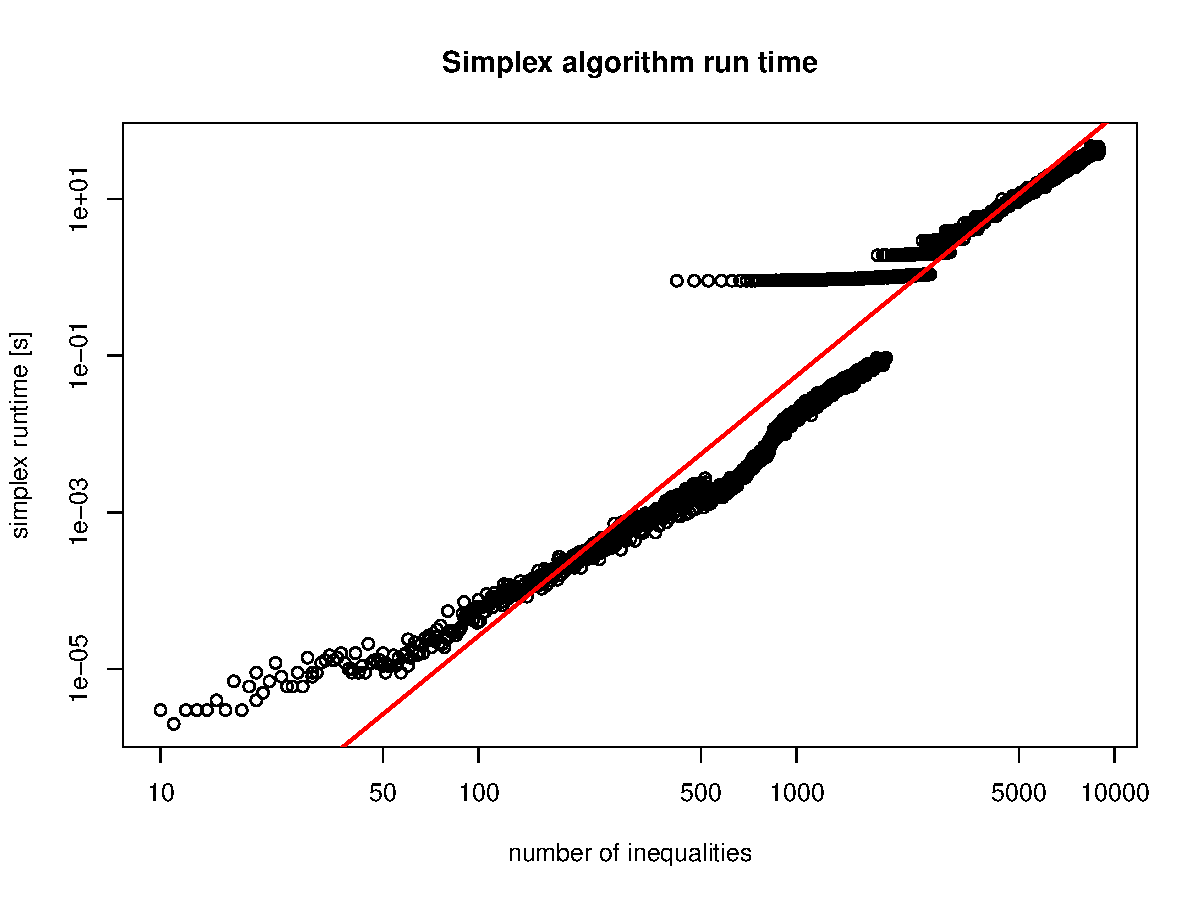
\includegraphics[width=\hsize]{add/runtime.pdf}
\end{center}
\caption{Laufzeit des Simplex-Algorithmus in der BLAS-basierten
Implementation\label{simplex:runtime}}
\end{figure}
In Abbildung~\ref{simplex:runtime} ist  die Laufzeit des Simplex-Algorithms
in der BLAS-basierten Implementation dargestellt.  Auffallend
ist das sprunghaft sich "andernde Verhalten der L"osung bei ungef"ahr
$n\simeq 1000$. Bei dieser Problemgr"osse umfasst die Matrix
ungef"ahr 8MB, m"oglicherweise wird hier die Cachegr"osse des
verwendeten Prozessors ausgesch"opft.

Interessant ist auch die Anzahl der Austauschschritte, die f"ur die
L"osung n"otig sind. 
\begin{figure}
\begin{center}
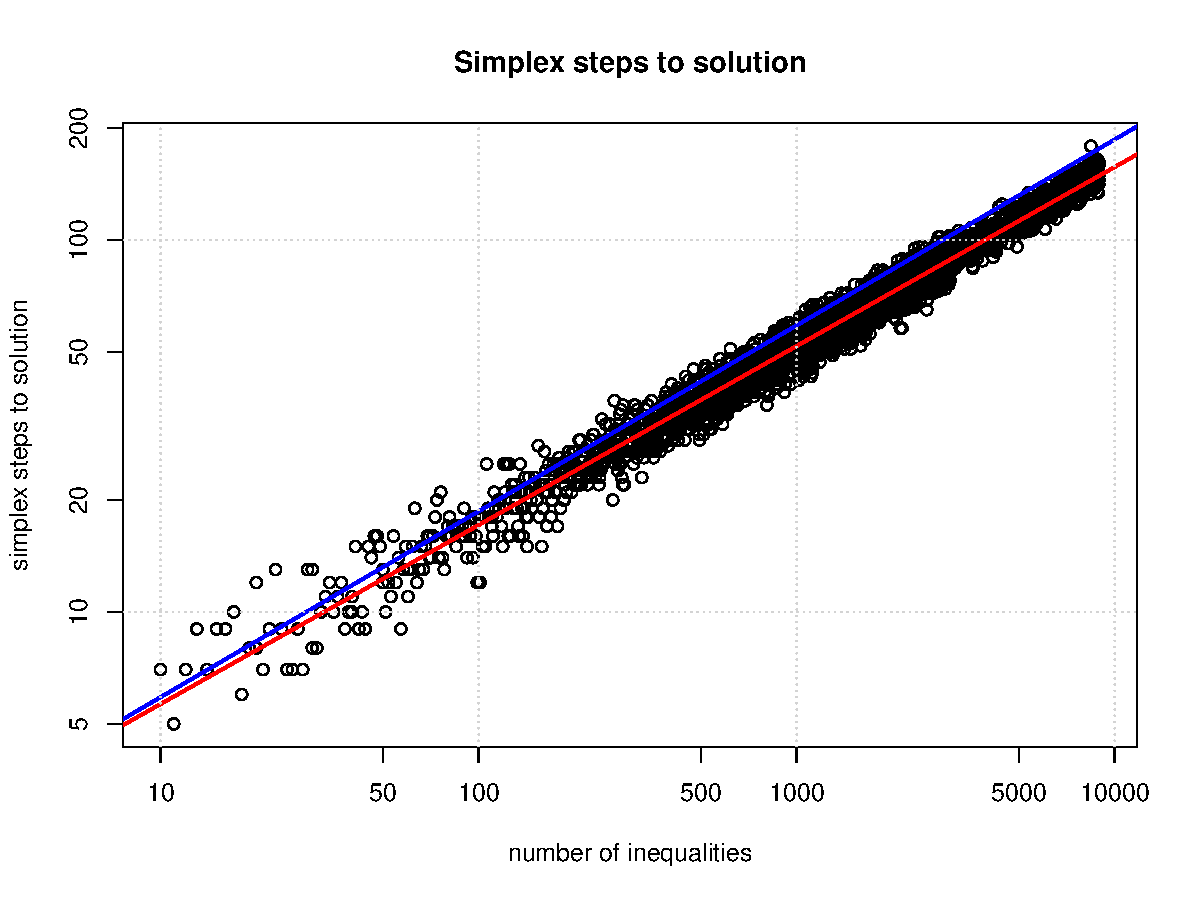
\includegraphics[width=\hsize]{add/pathsteploghyp.pdf}
\end{center}
\caption{Anzahl Schritte bis zur L"osung des Simplex-Algorithmus
in logarithmischer Darstellung.
Blau die Hypothese $\sim\sqrt{n}$.
\label{simplex:pathsteps}}
\end{figure}
Abbildung~\ref{simplex:pathsteps} zeigt die Anzahl Austauschschritte bis
zum Erreichen des Optimums. Die f"ur das Beispiel
verwendeten $n$ Ungleichungen zerlegen die Oberfl"ache einer Kugel in
$n$ Teile, von denen ein Weg des Simplex-Algorithmus ungef"ahr 
$O(\sqrt{n})$ treffen m"usste. In Wahrheit ist der Simplex-Algorithmus
sogar noch etwas effizienter.

\section{Wahl des Weges}
Die Wahl des Weges, den der Simplex-Algorithmus w"ahlt, wurde mit
mit Hilfe von graphischen Darstellungen ebenfalls untersucht.
Zun"achst f"allt in der Abbildung \ref{simplex:kanten} auf,
dass der Algorithmus nicht den direktesten Weg nimmt. Im ersten
Schritt findet er vom Ursprung aus den Schnittpunkt der $z$-Achse mit
dem Rand. Dann folgt er der Koordinatenebene bis ca.~$45^\circ$
n"ordlicher Breite, erst von dort folgt er den Kanten bis zum Maximum.
\begin{figure}
\begin{center}
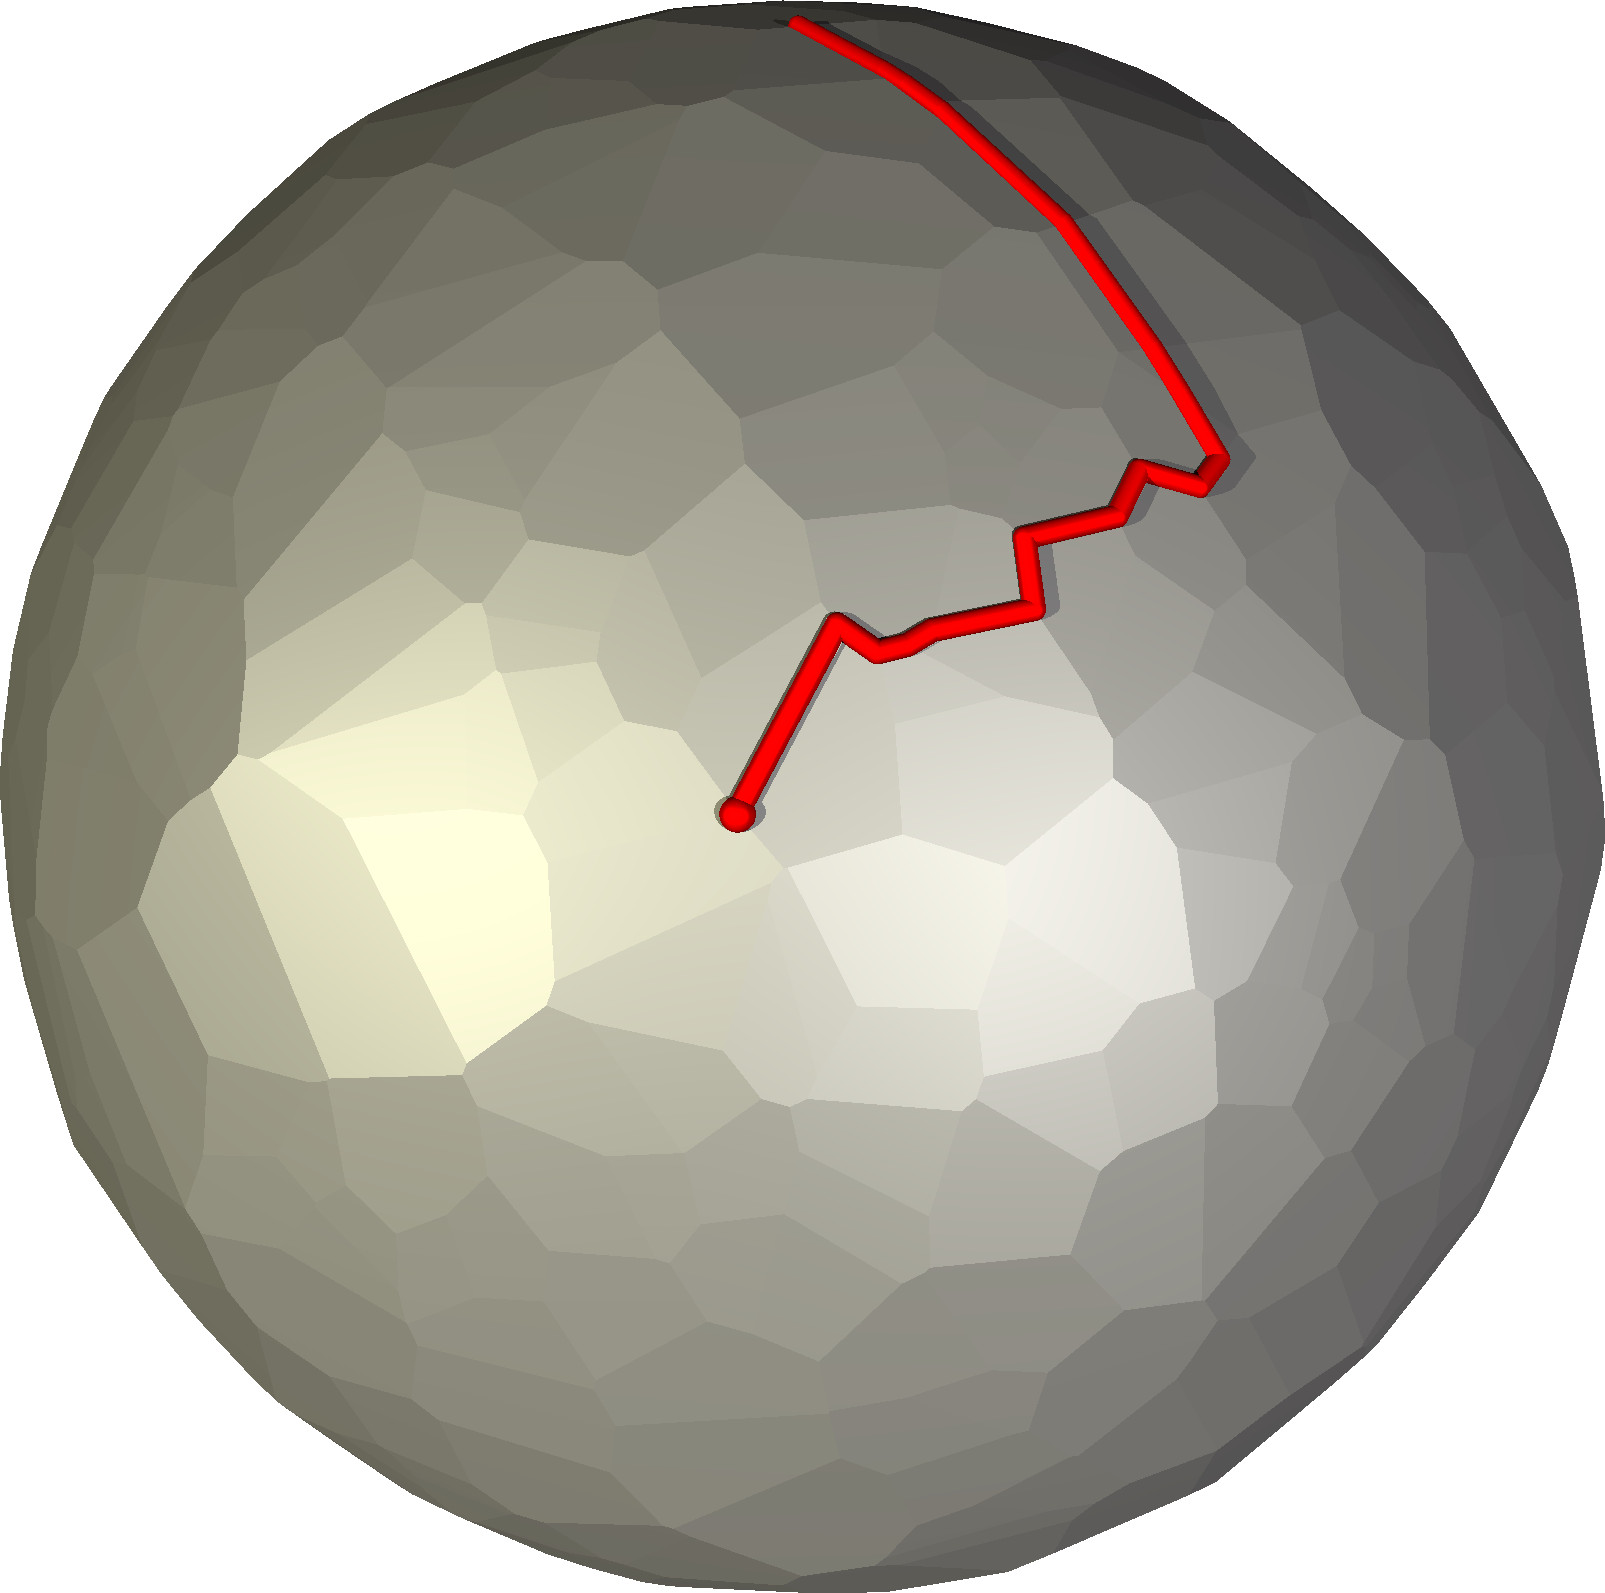
\includegraphics[width=0.7\hsize]{add/sphere.jpg}
\end{center}
\caption{Weg des Simplex-Algorithmus entlang der Kanten 
des zul"assigen Gebietes.
\label{simplex:kanten}}
\end{figure}
Weitere Beispiel in den Animationen auf Youtube:
\url{http://www.youtube.com/watch?v=54blxYi5JF8}
und
\url{http://www.youtube.com/watch?v=k9em_7B6298}.
Die zweite Animation zeigt, dass dieses z"ogerliche Vorgehen nicht
ein Zufall in Abbildung~\ref{simplex:kanten} ist, sondern das
generelle Verhalten des Algorithmus.
\section{Alternative Ans"atze}
Eine eigene Implementation des Simplex-Algorithmus ist oft nicht
notwendig, so kann man in Open Source Projekten oder in Projekten,
deren Programme nicht weiterverbreitet werden, das GNU Linear
Programming Toolkit (GLPK) verwenden, welches ausser dem
Simplex Algorithmus f"ur lineare Optimierung auch Methoden f"ur
ganzzahlige Optimierung und innere Punktmethoden beinhaltet.
